\section{Consideraciones iniciales}

El presente trabajo utiliza la norma APA 6ª edición para la citación de referencias bibliográficas. Todas las citaciones a lo largo del texto utilizan hipervínculos hacia sus entradas correspondientes en \emph{Referencias bibliográficas} de la página~\pageref{chap:referencias}. Gran parte de los términos científicos utilizados se encuentran en inglés y no se han traducido al español, ya que son ampliamente conocidos y usados en su forma original inglesa en el ámbito científico hispanohablante. De forma consistente, todos ellos están escritos en cursiva. Los términos utilizados repetidamente a lo largo del texto se encuentran en forma de acrónimos, los cuales son explicitados en su primer uso. El significado de estos acrónimos puede consultarse en el glosario de la página~\pageref{chap:glosario}, al cual apuntan todos ellos por medio de hipervínculos.

Eventualmente, se incluyen códigos QR que enlazan a vídeos, audios u otros recursos de interés (por ej., en la Figura \ref{fig:chatgpt_zero_shot_vs_few_shot}). Estos códigos pueden ser escaneados con cualquier dispositivo móvil, aunque también incluyen enlaces para su acceso desde el propio lector de PDF. Estos recursos son accesorios al texto y pueden cambiar o desaparecer con el tiempo. Por ello, en el Anexo \ref{anexo:repositorio} se incluye un enlace al repositorio de \emph{Github} donde se aloja el código fuente de este trabajo, escrito en \defaultLaTeX{}, y la versión actualizada de este PDF.

Por último, el título de este trabajo, hace un guiño a las ya cientos de publicaciones científicas que utilizan la expresión \emph{All You Need} en el título, como se puede observar en la Figura \ref{fig:all_you_need_publicaciones}. Esta expresión se ha convertido en un icono de los avances en inteligencia artificial especialmente desde la conocidísima publicación del artículo \emph{Attention Is All You Need} \citep{vaswaniAttentionAllYou2017} El lector curioso puede encontrar una lista actualizada de estas publicaciones en el repositorio \emph{Awesome "all you need" papers} \citep{nishiKentoNishiAwesomeallyouneedpapers2024}.


\begin{figure}[H]
    \caption[Número de publicaciones científicas del campo de la inteligencia artificial por año que contienen la expresión <<All You Need>> en su título]{Número de publicaciones científicas del campo de la inteligencia artificial por año que contienen la expresión <<All You Need>> en su título.}
    \centering
    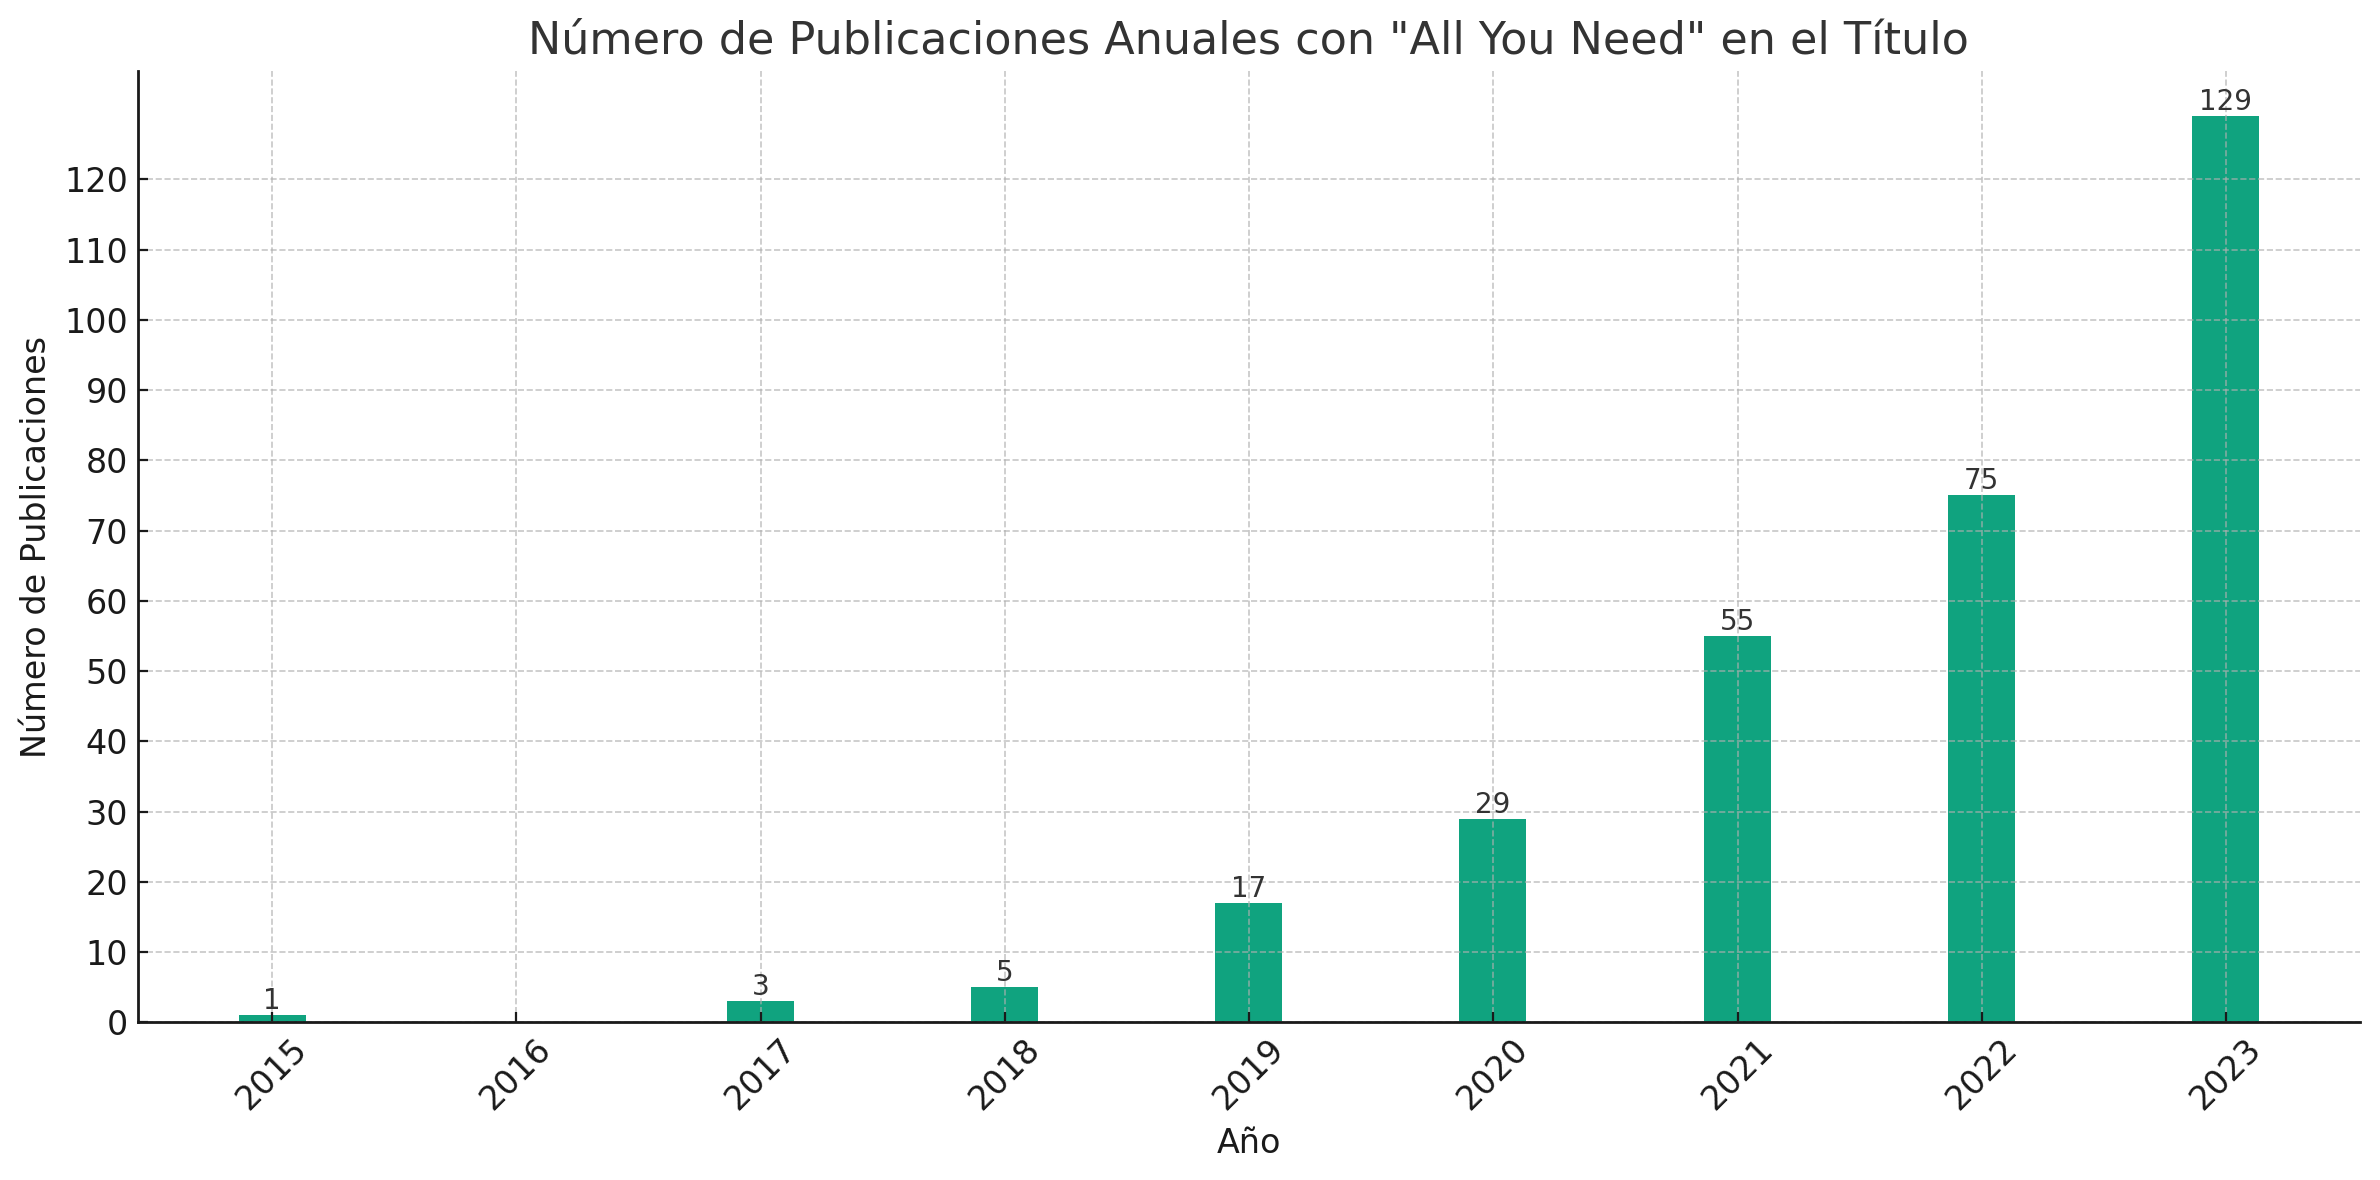
\includegraphics[width=0.7\textwidth]{./figuras/all_you_need_publicacionies_anuales.png}
    \source{\propio\ a partir del listado de \cite{nishiKentoNishiAwesomeallyouneedpapers2024}}
    \label{fig:all_you_need_publicaciones}
\end{figure}



